% This is LLNCS.DEM the demonstration file of
% the LaTeX macro package from Springer-Verlag
% for Lecture Notes in Computer Science,
% version 2.4 for LaTeX2e as of 16. April 2010
%
\documentclass{llncs}
%
\usepackage{makeidx}  % allows for indexgeneration
%
\usepackage{graphicx}
\graphicspath{ {images/} }
\begin{document}
%
\frontmatter          % for the preliminaries
%
\pagestyle{headings}  % switches on printing of running heads

\mainmatter              % start of the contributions
%
\title{Anomaly Detection Challenges - Challenge III}
%
\titlerunning{Challenge 3}  % abbreviated title (for running head)
%                                     also used for the TOC unless

%
\author{Hamza Tahir (03670002) \and Muhammad Hamza Usmani (03669506)}
%
\authorrunning{Tahir \and Usmani} % abbreviated author list (for running head)
%
\institute{Technical University of Munich}
%%%% list of authors for the TOC (use if author list has to be modified)

\maketitle              % typeset the title of the contribution


%
\section{Introduction}
%
This brief report serves as a purpose to present and explain the methodologies applied to tackle the third challenge in the Practical: Anomaly Detection Challenges. Section~2 discusses the challenge task and the data set for the machine learning/anomaly detection task. Section~3 explains the approaches adopted for the task.
%
\section{The Challenge}
%
%
\subsubsection{Machine Learning Task}
%
The machine learning task for this challenge is to determine if a network trace is a normal transaction or an attack.
\begin{table}
\caption{Decision Classes}
\begin{center}
\begin{tabular}{r@{\quad}rl}
\hline
\multicolumn{1}{l}{\rule{2pt}{0pt}
Class}&\multicolumn{2}{l}{Representation}\\[2pt]
\hline\rule{0pt}{12pt}
Normal&    1& \\
Attack&     0& \\[2pt]
\hline
\end{tabular}
\end{center}
\end{table}
%
\subsubsection{The Data set}
The dataset consists of network traces. There are 56,041 records in the training set with 43 network related features. The training dataset consists of 56,000 normal records and 41 attack rows, the attack rows consist of 9 different attack types, the machine learning task however for this challenge is to classify a record as attack or normal.

\section{Methodology}
This section explains the data analysis and the machine learning process to build the model for classifying the given samples as attack  or normal record. 

\subsection{Machine Learning Based NIDS}
One of the most common reasons that machine Learning based network intrusion detection techniques are challenging is because of it is an outlier detection technique \cite{Garcia:etal}, this challenge is even more difficult because of very few attack records in the training set, that have 9 different attack types, making it difficult to develop a profile of the attack behavior.

\subsection{Data Visualization}
To select classification techniques and to better analyze the data, a technique that the authors used is data visualization. Since the original data set is in high dimensional space, techniques were used to reduce the dimensions to visualize the attack and normal records. t-distributed Stochastic Neighbor Embedding (TSNE) was used to reduce the dimension of the data to two basic features, and subsequently sample points were plotted. TSNE converts similarities between data points to joint probabilities and it tries to minimize the Kullback-Leibler divergence between the joint probabilities. The visualized attacks and selected normal data are shown in Figure 1 and 2.

\begin{figure}
  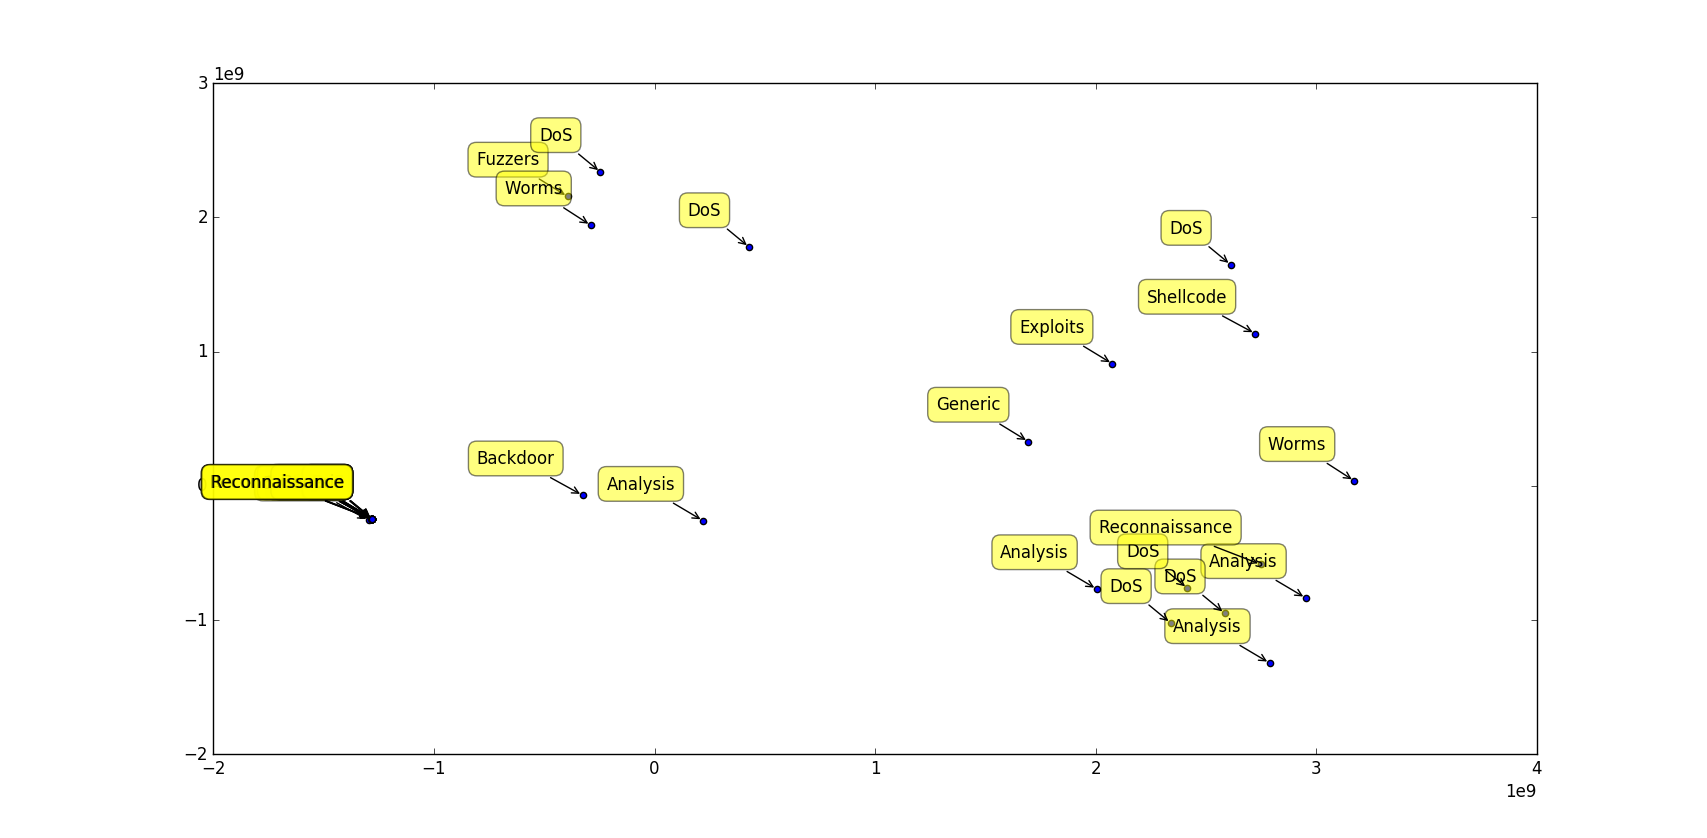
\includegraphics[width=\linewidth]{anamolies_tsne.png}
  \caption{Anomalies in reduced space}
  \label{fig:anomalies_tsne}
   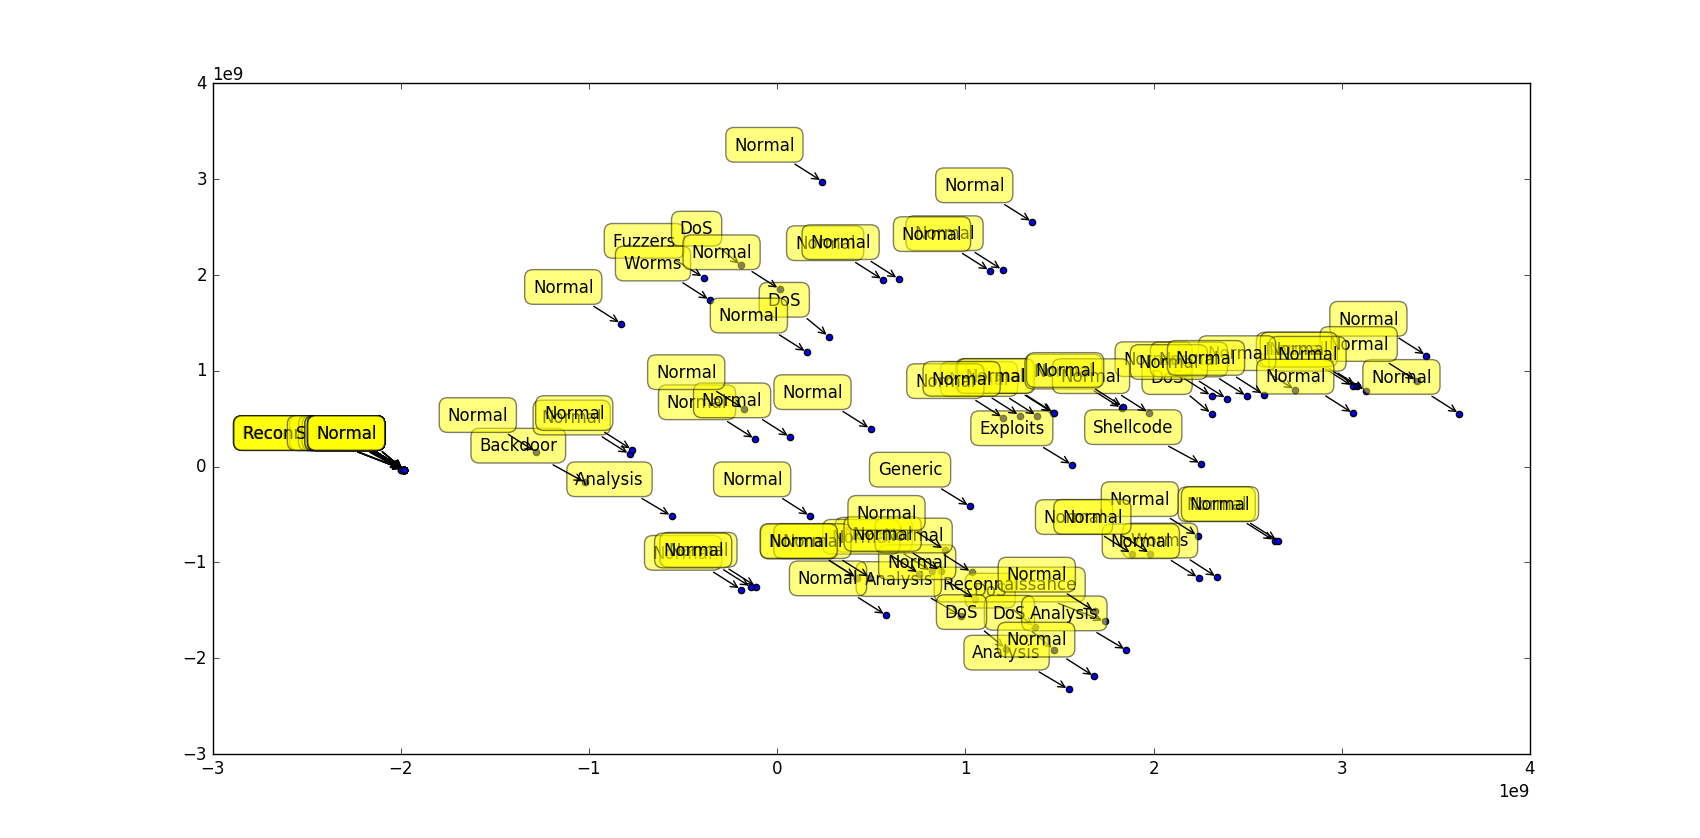
\includegraphics[width=\linewidth]{anamolieswithnormal_tsne.png}
  \caption{Anomalies and Selected Data in reduced space}
  \label{fig:anomalies_data_tsne}
\end{figure}

As is evident from the projected, reduced space, the data is not easily separable (at least in this approximation).
\subsection{Feature Scaling}
The given features and the extended behavioral features have different scales, this required to normalize all features on one scale, so that the different ranges and scales of features do not contribute to relative weights of those features. To normalize, the following method was used:
\[ X^{'} =\frac{X - X_{min}}{X_{max} - X_{min}}   \]

\subsection{Re-sampling}
The training data set is higher number of normal network traffic in comparison to attack records, thus the data was re-sampled to build a robust classifier. The re-sampled data set had 40 normal records that were randomly chosen from the data set, and 41 fake records from the training data set.

\subsection{Machine Learning Techniques}
Following supervised and unsupervised machine learning techniques were used to classify given samples as "Normal" (represented as 0) or "Attack"(represented as 1):
\begin{enumerate}
   \item Random Forest (Supervised)
   \item KNN Classifier (Unsupervised)
   \item Logistic Regression (Supervised)
   \item KNN Regressor (Semi-Supervised)
 \end{enumerate}
 
\subsection{Generalizing - Developing a Robust Classifier}
To build a robust classifier, that is relatively general and is not restricted only to the given training set following techniques were used:

\subsubsection{Three-fold Cross Validation:} Three-fold cross validation was used to overcome the problem of over-fitting, and to build a model to that will generalize to an independent dataset, Hawkins et. al. (see \cite{hawkins:eke}).  


\section{Results}
Results of the challenge are summarized in this section. We present results based upon training accuracies only. The results presented are achieved after feature scaling and random re-sampling and three-fold cross validation.

\begin{table}
	\centering
	\caption{Best Average Cross-Validation Accuracies}
	\begin{tabular}{ |p{3cm}||p{3cm}||p{3cm}|}
		\hline
		Technique                  &Training Accuracy &Testing Accuracy\\
		\hline
		Random Forest              &91.347 &82.063\\
		KNN Classifier             &87.224 &77.319\\
		KNN Regressor              &88.892 &74.669\\
		Logistic Regression        &92.119 &71.958\\
		\hline
		 Average     &\textbf{87.948} &\textbf{76.503}\\
		 \hline
	\end{tabular}
	\label{table}
\end{table}

As you can see, there is quite a big gap between training and test accuracies. This can be explained due to the fact that we used a very small sample for our classifier, due to the under sampling and the fact that there are only about 50 anomalous entries. This would make our k-fold classification approach tend to overfit. 

As we examined the data, we tried to project the anomalies to 2D space to visualize it. We can see the result in Fig. 1, where we only plot anomalies and Fig. 2 where we also plot it with some normal points. As it can be seen, there is no obvious separation in this space between anomalous and normal entries. However, we did observe some anomalous entries were groped together in terms of their attack categories. Therefore, we decided to use an semi-supervised clustering approach to try to cluster the anomalies together, and then extrapolate the testing set from that. We used a KNN regressors approach. 

However, this approach did not fair any better than the supervised Random Forest approach which scored the best out of all classifiers. 

%
% ---- Bibliography ----
%
\begin{thebibliography}{5}
%
\bibitem{Garcia:etal}
P. Garcı´a-Teodoroa, J. Dı´az-Verdejoa, G. Macia´-Ferna´ndeza, E. Va´zquezb.
Anomaly-based network intrusion detection: Techniques, systems and challenges
aDepartment of Signal Theory, Telematics and Communications – Computer Science and Telecommunications Faculty,
University of Granada, Granada, Spain (2008)
\bibitem {hawkins:eke}
Hawkins D. , Basak S. , and Denise M. 
Assessing Model Fit by Cross-Validation
J. Chem. Inf. Comput. Sci., 2003, 43 (2), pp 579–586 (2003)

\end{thebibliography}
\end{document}
